% DESCRIÇÃO DA PROPOSTA--------------------------------------------------------------------


\chapter{INTRODUÇÃO}
\label{chap:introducao}

% Introdução-------------------------------------------------------------------------------
% (máximo de 1 página)
Nos anos recentes, foi notado um grande aumento no tráfego e armazenamento de diferentes aplicações e dados multimídias, como imagens, áudio, vídeo, impressões digitais, séries temporais,
sequências de proteínas, etc. Estes tipos de dados, que apresentam muito mais atributos do que simples numerais ou pequenas cadeias de caracteres, são conhecidos como dados complexos \cite{Zighed2008}.\par
Quando tratados por um Sistema Gerenciador de Banco de Dados Relacional (SGBDR), não suportam comparações com os operadores conhecidos como "big six"\ da linguagem SQL: $=$, $\neq$ , $<$, $>$, $\leq$, $\geq$.
Esse fato limita muito as comparações entre dados complexos inseridos em um SGBDR, ocasionando um grande problema no contexto de base de dados, uma vez que os principais sistemas de gerenciamento
de base de dados são relacionais \cite{DBE2017}. Com isso, tornou-se necessária a concepção de novos tipos de comparadores, como buscas por similaridade.\par 

Estas consultas por similaridade se aplicam de maneira geral a muitos dos tipos de dados complexos \cite{Barioni2009}. Embora equiparar duas imagens médicas (como tomografias de pacientes distintos) 
raramente produza um resultado diferente de falso, procurar por imagens semelhantes à original faz mais sentido e retorna resultados mais relevantes. Dentre os operadores de consulta por similaridade
os mais comuns são as consultas por abrangência (\textit{range query: Rq}) e consulta aos k-vizinhos mais próximos (\textit{k-nearest neighbor querry: kNNq}). As consultas por abrangência \textit{Rq($s_q$, $\xi$)}
recebem como parâmetro um elemento $s_q$ do domínio de dados (elemento central da consulta) e um limite máximo de dissimilaridade $\xi$. O resultado é o conjunto de elementos da base que diferem do elemento
central da consulta por no máximo a dissimilaridade indicada.\par

\begin{figure}[ht]
\centering
\captionsetup{width=0.50\textwidth, font=footnotesize, textfont=bf}
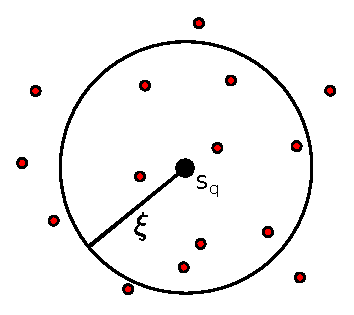
\includegraphics[width=.3\textwidth]{dados/figuras/rq.eps}
\caption{Exemplo de consulta por abrangência}
\label{fig:exemplorq}
\end{figure}


Uma consulta aos k-vizinhos mais próximos \textit{kNNq($s_q$, $k$)} também recebe como um de seus parâmetros um elemento central da consulta $s_q$, e um número inteiro $k$ de vizinhos desejados, e retorna
como resultado o conjunto dos $k$ elementos com a menor dissimilaridade em relação ao elemento central da consulta $s_q$ \cite{POLA2010}.
\newpage
\begin{figure}[ht]
\centering
\captionsetup{width=0.50\textwidth, font=footnotesize, textfont=bf}
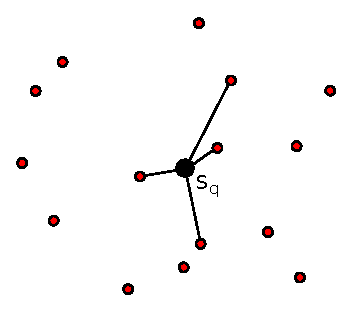
\includegraphics[width=.3\textwidth]{dados/figuras/knnq.eps}
\caption{Exemplo de consulta por k-vizinhos mais próximos}
\label{fig:exemploknnq}
\end{figure}

O SGBDR não possui suporte nativo a estes tipos de consulta, mas é possível construir estas consultas utilizando ferramentas existentes em um banco de dados relacional (como a \textit{B-tree}).
Para entender e ajustar os métodos de consultas por similaridade para diferentes tamanhos e tipos de conjuntos de dados, além de comparar diversos métodos, é importante uma análise teórica dos diferentes
métodos de acesso e técnicas de estimativa do custo computacional \cite{POLA2010}. O cálculo do custo das operações realizadas será feito utilizando operações com B-trees, as quais o banco fornece suporte
ao modelo de custo.

A solução abordada por esta proposta é a do uso de técnicas Omni, presentes no trabalho de \cite{Traina2001}. Um número calculado de elementos do conjunto de dados são selecionados como "focos", e utilizados para
podar cálculos desnecessários de distâncias, fazendo uso da desigualdade triangular. Para quaisquer elementos $s_1$, $s_2$, $s_3$ $\in$ $\mathbb{S}$, sendo $\mathbb{S}$ um domínio de elementos
e uma métrica $d : \mathbb{S} \times \mathbb{S} \rightarrow \mathbb{R^+}$, temos a desigualdade triangular:

\begin{equation} \label{eq:destri}
		d(s_1,s_2) \leq d(s_1,s_3) + d(s_3,s_2)
\end{equation}
\par

A base da técnica Omni é calcular previamente as distâncias de todos os elementos para todos os focos selecionados, armazenando estas distâncias no banco. Quando uma consulta por similaridade
(como uma consulta por abrangência) é realizada, são conhecidas as distâncias entre o elemento central da consulta $s_q$ e o raio de abrangência $\xi$. Considerando um foco ${f_1}$ e utilizando
a desigualdade triangular, elementos que possuem uma distância entre o foco escolhido menor do que a distância de $s_q$ até o foco menos o valor $\xi$ serão descartados do conjunto de elementos necessários para
os cálculos de distância com o elemento central. Simetricamente, elementos cuja distância até o foco seja maior do que a distância de $s_q$ até o foco mais o valor do raio de abrangência $\xi$ também
serão descartados. Com isso, ocorre uma grande redução do número de cálculos necessários para fornecer o conjunto resposta. Essa poda também pode ser realizada por mais de um foco.

\begin{figure}[H]
\centering
\captionsetup{width=0.50\textwidth, font=footnotesize, textfont=bf}
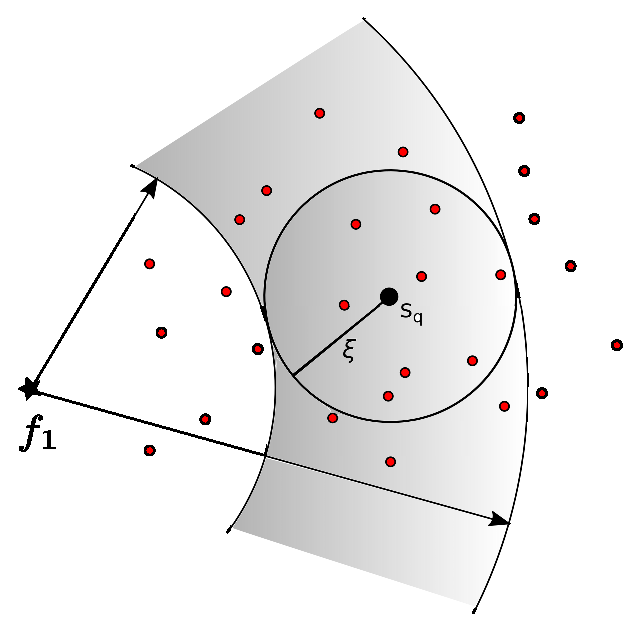
\includegraphics[width=.4\textwidth]{dados/figuras/rg_omni_1.eps}
\caption{Consulta por abrangência pela técnica Omni utilizando um foco}
\label{fig:rqomni1}
\end{figure}


A figura \ref{fig:rqomni1} ilustra a poda no número de cálculos. Apenas os elementos na área sombreada terão as suas distâncias em relação ao centro da consulta calculadas, pois estão no
conjunto de elementos que não foram descartados utilizando a desigualdade triangular com as distâncias previamente calculadas em relação ao foco. O armazenamento das distâncias de cada foco ${f_i}$ para cada outro elemento $s_k$ será feito 
utilizando uma estrutura de indexação que implementa os conceitos da técnica Omni com a estrutura da B$^+$-tree, originando uma nova estrutura chamada de Omni-Btree. As distâncias serão armazenadas em $l$ Omni-Btrees, sendo $l$ o número de focos
criados para a base de dados \cite{Traina2001}.

O principal foco deste trabalho é o emprego destas técnicas para bases de dados constituídas por imagens. Para isto, torna-se necessário o uso de uma miríade de extratores de características
das imagens, para um maior refinamento do uso de consultas por similaridade. Estas características podem se referir a: atributos visuais (cor, forma, textura), atributos lógicos (identificação
de elementos) e atributos semânticos (identificação de emoções humanas). As características visuais podem ser utilizadas como histogramas de cores para a análise de cor, matrizes de co-ocorrência para a análise de textura e
métodos baseados em contorno para a análise de forma. Geralmente, consultas são feitas utilizando uma combinação destas características, e não apenas uma delas.
\\ \\

%-----------------------------------------------------------------------------------------
{\let\clearpage\relax \chapter{OBJETIVOS}}
\label{chap:objetivos}
% (máximo de 1/2 página)

O objetivo geral deste trabalho é elaborar um sistema de que seja capaz de realizar consultas por similaridade em uma base de dados complexos, mais precisamente em um conjunto de imagens.
Estas imagens podem variar de fotografias de ambientes, rostos de pessoas, impressões digitais e imagens de diagnósticos médicos como radioagrafias e tomografias, por exemplo.
A ideia central é implementar todo o mecanismo de armazenamento, cálculo de distâncias e busca de dados similares no próprio banco de dados, deixando apenas a interface com o usuário fora do banco.

Após as etapas de povoamento do banco e implementação das consultas estiverem concluídas, será criada uma interface gráfica para facilitar o acesso do usuário com o sistema de consulta. Também serão
estudadas maneiras de se otimizar estas consultas, utilizando diferentes métodos e formas de indexação dos elementos dentro do banco. \\ \\


%-----------------------------------------------------------------------------------------

{\let\clearpage\relax \chapter{MATERIAIS E MÉTODOS}}
% \chapter{METODOLOGIA} % Escolher o nome mais adequado ao trabalho
\label{chap:matmetodos}

% Procedimentos Metodológicos/Metodologia-------------------------------------------------
% (máximo de 2 páginas)
O SGBDR utilizado será o PostgreSQL, um sistema de gerenciamento de banco de dados objeto-relacional gratuito e de código-aberto. Os extratores de características das imagens utilizados são do framework Arboretum, desenvolvido
pelo Grupo de Bases de Dados e Imagens (GBDI) da Universidade de São Paulo - campus São Carlos. Para a interface com o usuário, será estudado um framework que atenda as necessidades deste trabalho. \\ \\

% 
% Na seção de procedimentos metodológicos ou metodologia (ver qual o nome mais adequado ao trabalho) deve ser descrito sucintamente o procedimentos metodológicos para a execução do projeto ressaltando como os objetivos serão alcançados. 
% 
% Em geral, a seção descreve os procedimentos usados para resolver o problema atacado. Pode ser estruturada em tópicos, onde cada tópico representa um subproduto do objetivo geral.
% 
% No caso de desenvolvimento de sistemas deve-se descrever a metodologia a ser utilizada, por exemplo Scrum, eXtreme Programming, RUP, etc. 
% 
% Também pode ser descritos técnicas de desenvolvimento de software como por exemplo TDD, BDD, SPA,  etc.
% 
% (substitua este texto pelo de procedimentos metodológicos/metodologia do trabalho)
% %-----------------------------------------------------------------------------------------



 
{\let\clearpage\relax \chapter{CONCLUSÃO}} % Escolher o nome mais adequado ao trabalho
\label{chap:conclusao}
% Conclusão/Considerações Finais----------------------------------------------------------
% (máximo de ½ página)

Ao término deste trabalho, espera-se que o aluno tenha obtido domínio sobre o SGBD PostgreSQL e suas ferramentas, assim como um maior entendimento e experiência no campo de estudos de dados complexos.
Após o sistema ser concluído, será possível a implementação de um sistema de recuperação de imagens baseado em conteúdo (\textit{Content-Based Image Retrieval - CBIR}). Com isto, espera-se utilizar
este CBIR para o gerenciamento de imagens médicas, um campo onde há uma produção crescente de imagens utilizadas em diagnósticos e terapias. Técnicas utilizadas em diagnósticos como raciocínio baseado
em casos necessitam fortemente de recuperação de imagens por semelhança, o que pode ser valioso para suportar certos diagnósticos médicos \cite{Long2009}. \\ \\


%-----------------------------------------------------------------------------------------

 
 
{\let\clearpage\relax \chapter{CRONOGRAMA}}
\label{chap:cronograma}

%Estudo, modelagem, verificação das estruturas Omni, bases, extratores, métricas, criar o banco e inserir as métricas, implementação da Omni, implementação seq sem Omni, comparação
% Planejamento do Trabalho----------------------------------------------------------------
% Esta seção não precisa ser editada, apenas edite o quadro 1 armazenada no diretório ".\dados\quadros"

\begin{quadro}[!htb]
    %\centering
    \caption{Cronograma de Atividades.\label{qua:cronograma}}
    \begin{tabular}{|p{5.0cm}|p{0.6cm}|p{0.6cm}|p{0.6cm}|p{0.6cm}|p{0.6cm}|p{0.6cm}|p{0.6cm}|p{0.6cm}|p{0.6cm}|p{0.6cm}|}
        \hline
        \textbf{Atividades} 						     & 	   \textbf{Set}      & \textbf{Out} & \textbf{Nov} & \textbf{Dez} & \textbf{Jan} & \textbf{Fev} & \textbf{Mar} & \textbf{Abr} & \textbf{Mai} & \textbf{Jun} \\
        \hline
        \footnotesize{1. Estudo e acompanhamento da literatura}		     & X	             & X            &  		   & 		  &  		 &   	        &   	       &   	      & 	     & 		     \\
        \hline
        \footnotesize{2. Modelagem do problema} 				     & X	             & X            &  		   & 		  &  		 &   	        &   	       &   	      & 	     &                \\
        \hline
	\footnotesize{3. Verificação das estruturas Omni} 			     &  	             & X            & X		   & 		  &  		 &   	        &   	       &   	      & 	     &                \\
        \hline
	\footnotesize{4. Estudo dos extratores de características} 		     &  	             &              & X		   & 		  &  		 &   	        &   	       &   	      & 	     & 		     \\
        \hline
	\footnotesize{5. Estudo e inserção das métricas no banco} 		     &  	             & X            & X		   &  		  &  		 &   	        &   	       &   	      & 	     & 		     \\
        \hline
	\footnotesize{6. Criação e povoamento da base de dados} 		     &  	             &              & X		   & X		  &  		 &   	        &   	       &   	      & 	     & 		     \\
        \hline
        \footnotesize{7. Elaboração da apresentação do TCC1}			     &  	             &              & X		   & X		  &  		 &   	        &   	       &   	      & 	     & 		     \\
        \hline        
        \footnotesize{8. Defesa do TCC1}                                             &  	             &              &  		   & X		  &  		 &   	        &   	       &   	      & 	     & 		     \\
        \hline
	\footnotesize{9. Implementação da busca sequencial} 			     &  	             &              &  		   & 		  & X		 & X	        & X 	       &   	      & 	     & 		     \\
        \hline
        \footnotesize{10. Implementação da técnica Omni} 			     &  	             &              &  		   & 		  & X		 & X 	        & X 	       &   	      & 	     & 		     \\
        \hline
        \footnotesize{11. Comparação e análise de resultados} 			     &  	             &              &  		   & 		  &  		 &   	        &  X	       & X 	      & 	     & 		     \\
        \hline
        \footnotesize{12. Implementação da interface} 				     &  	             &              &  		   & 		  &  		 &   	        &  X	       &  X	      & 	     & 		     \\
        \hline
        \footnotesize{13. Elaboração da apresentação final} 			     &  	             &              &  		   & 		  &  		 &   	        &   	       &  X	      &  X	     & 		     \\
        \hline        
        \footnotesize{14. Defesa do TCC2}					     &  	             &              &  		   & 		  &  		 &   	        &   	       &   	      & 	     & X	     \\
        \hline
    \end{tabular}
\end{quadro}

%Estudo, modelagem, verificação das estruturas Omni, bases, extratores, métricas, criar o banco e inserir as métricas, implementação da Omni, implementação seq sem Omni, comparação
%-----------------------------------------------------------------------------------------
